\documentclass[11pt,a4paper]{report}
\usepackage[utf8]{inputenc}
\usepackage[german]{babel}
\usepackage{amsmath}
\usepackage{amsfonts}
\usepackage{amssymb}
\usepackage{graphicx}
\usepackage{fancyhdr}
\usepackage{geometry}
\usepackage{nameref}
\geometry{a4paper, left=25mm, right=25mm, top=20mm, bottom=30mm}

\renewcommand{\headrulewidth}{1pt} % Trennunslinien für Kopf- und Fußzeilen
\renewcommand{\footrulewidth}{1pt}

\lhead{LAN-Monitoring} % Kopf- und Fußzeilen
\rhead{\chaptername \hspace{5mm} \thesection}
\lfoot{Du hasch deinen Namen vergessen}
\rfoot{\thepage}

\title{MAD-Network Monitoring\\
Diplomarbeit 2014/15}
\author{Porcic Alin, Ranalter Daniel, Singh Manpreet, Stojanovi\'{c} Marko\\
Betreuer: Dr. Michael Weiss\\
Höhere Technische Bundes Lehr- und Versuchsanstalt Anichstraße\\
Abteilung Höhere Elektronik und Technische Informatik\\
5bHEL}

\begin{document}
\maketitle
\newpage

%\setcounter{tocdepth}{6}
\tableofcontents
\newpage

\pagestyle{fancy}
\part{Abstract}
\chapter{Abstract}
\thispagestyle{fancy}

lorem ipsum

\part{Einleitung}
\thispagestyle{fancy}

lorem ipsum

\chapter{Aufgabenstellung}
lorem ipsum

\chapter{Aufteilung}
lorem ipsum 

\part{Theorie zu den einzelnen Gebieten der Arbeit}
lorem ipsum

\chapter{Informatik von Stojanovic Marko}
lorem ipsum

\section{Programmiersprachen}
lorem ipsum
\subsection{Was ist eine Programmiersprache?}
lorem ipsum
\subsection{C\#}
lorem ipsum
\subsubsection{Wie funktioniert C\#}
lorem ipsum
\subsubsection{Vor- und Nachteile}
lorem ipsum
%\subsection{Vergleich anderer möglicher Programmiersprachen}
%lorem ipsum
\section{Multithreading}
lorem ipsum
\subsection{Was ist ein Thread}
lorem ipsum
\subsection{Konzept von Multithreading}
lorem ipsum
\subsubsection{Wie funktioniert Multithreading}
lorem ipsum
\subsubsection{Hardware}
lorem ipsum
\subsubsection{Software}
lorem ipsum
\subsubsection{Arten von Multithreading}
lorem ipsum
\subsubsection{Vor- und Nachteile}

\lfoot{Ranalter Daniel}
\chapter{Netzwerkgrundlagen und Protokolle von Ranalter Daniel}
Diese Abhandlung wird die Netzwerkgrundlagen welche auf das Ethernet Protokoll (siehe Kapitel \ref{ssec:eth}  Seite \pageref{ssec:eth}) aufsetzen besprochen. Es gibt noch diverse andere, wie zum Beispiel Token Ring, auf welche hier im folgenden jedoch nicht näher eingegangen wird, da, abgesehen davon, dass Ethernet auch bei der praktischen Durchführung verwendet wurde, Ethernet das am häufigsten genutzte Layer 1 Protokoll darstellt. 
\section{Grundlagen}
In der Netzwerktechnik gibt es mehrere verschiedene grundlegende Konzepte auf welche hier eingegangen werden soll.
\subsection{Netzwerkdevices}
Um ein Netzwerk aufzubauen werden verschiedene Devices benötigt. Je nach Größe und Art des Netzwerkes kann man auch auf einzelne Komponenten verzichten. 
\subsubsection{Router}
Ein Router kommt in so gut wie jedem Netzwerk vor. Er operiert auf dem Layer 3 im OSI-Schichtenmodell, indem er Packete welche an seine seiner Interfaces reinkommen, anhand der IP-Adresse an einem anderen Interface wieder hinaus schickt. Dadurch verbindet er logisch getrennte Netze.\\


\begin{figure}
\begin{center}
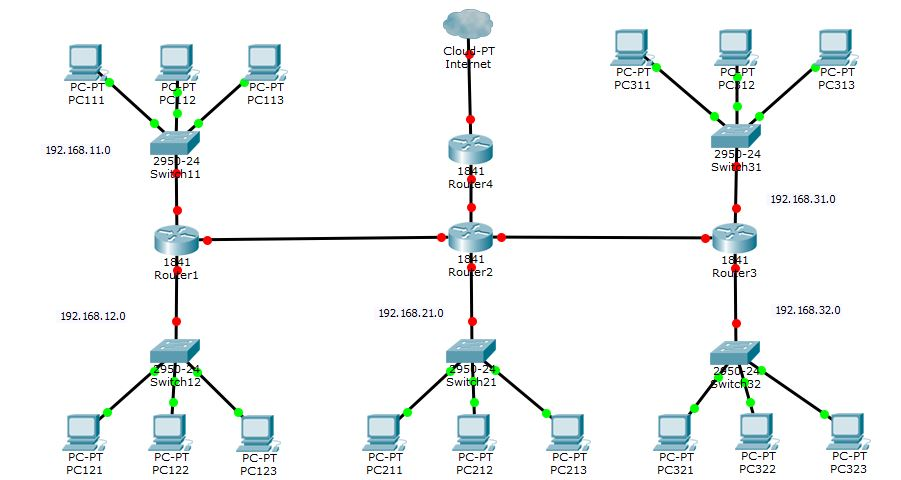
\includegraphics[scale=0.5]{../docs/tarkes/pics/RouterNetwork.jpg}\label{fig:bspNetwork}
\end{center}
\end{figure}


Das Wissen, welches Packet wohin muss, zieht er aus einer lokalen Routingtabelle. Diese Tabelle kann auf drei unterschiedliche Arten entstehen\\
\begin{itemize}
\item \textbf{Direkt angeschlossene Netze}\\
Netze welche direkt an einem seiner eigenen Interfaces hängen, erkennt er ohne weiteres zutun.\\
Auf dem Bild wären die Netze 192.168.11.0 192.168.12.0 und 192.168.22.0 dem Router1 also bekannt und er könnte Anfragen von Host121 an Host111 ohne Probleme weiterleiten.
\item \textbf{Statisches Routen}\\
Es ist dem Admin eines Netzwerkes möglich alle möglichen Routen von einem Netz zum anderen händisch am Router einzutragen.\\
Vorteilhaft daran ist die hohe Sicherheit und Kontrolle über das Netzwerk, nachteilig jedoch, dass es bei größeren Netzwerken sehr schnell unmöglich statisches routen anzuwenden da es sehr viel Arbeit darstellt jede mögliche Route händisch einzutragen ohne dabei einen Fehler zu machen.\\
Anhand des Bildes wäre es dem Administrator des Netzwerkes zum Beispiel möglich Router1 zu sagen, dass, wenn er zu Host212 kommen will, über das Netz 192.168.22.0 gehen muss. Was danach passiert, braucht Router1 nicht zu wissen, da sich nun Router2 um das Paket kümmern muss. Er erkennt, dass die Ziel IP-Adresse sich in einem direkt angeschlossenen Netz befindet, und schickt das Paket an dem entsprechenden Interface raus.
\item \textbf{Dynamisches Routen}\\
Beim dynamischen Routen lernt der Router anhand von eigenen Routing Protokollen wie er zu welchem Netz kommt. Es gibt einige verschiedene, welche alle verschiedene Prioritäten setzen. So versucht das Protokoll OSPF (Open Shortest Path First) immer so wenig Hops, also Netzwerkwechsel/Router, wie möglich passieren zu müssen. RIP (Routing Information Protocol) und dessen Nachfolger RIP2 werden zwar noch verwendet, aber als veraltet angesehen.
\end{itemize}

Des weiteren gibt es verschiedenste Arten von Routern. Ihre Grundfunktionalitäten sind zwar immer die gleichen, jedoch würde das kleine Kästchen das zuhause steht, nie ausreichen um den Traffic der Backboneleitungen, also der großen Glasfaserleitungen welche die Kontinente verbinden, zu routen. Dafür würde diesem Router einfach die Leistung fehlen.\\
Deshalb gibt es verschiedene Arten von Routern. Ein paar wichtige sind:\\
\begin{itemize}
\item Backbone-Router\\
Hochgradig auf Datendurchsatz optimiert, werden sie, wie der Name schon sagt, für das Routen an der Backbone verwendet.
\item Edge-Router, Border-Router\\
Wird von ISPs (Internet Service Providers wie UPC oder Telekom) verwendet um die Netzwerke ihrer Clienten zu verbinden. Sie verwenden normalerweise das Routing Protokoll BGP (Border Gateway Protocol) welches für diese Aufgabe ausgelegt ist.
\item WLAN-Router\\
Im Grunde ganz normale Router, welche jedoch zusätzlich die Möglichkeit besitzen nicht nur kabelgebunden zu kommunizieren sondern auf über das Funkband. In Österreich sind die Bänder 2,4 GHz und 5 GHz in Verwendung.
\item Customer-Edge-Router\\
Werden meistens von den ISPs den Kunden zur Verfügung gestellt. Die meisten unterstützen heutzutage auch WLAN.
\end{itemize}
\subsubsection{Switch}
Ein Switch ermöglicht die Kommunikation zwischen mehreren Hosts. Einfache Switches agieren hauptsächlich auf dem Layer2: Sie schreiben sich auf an welchem Port welche MAC-Adresse hängt und wissen dann durch Source und Destination MAC-Adresse, an welchen Interface das Paket wieder raus muss.\\

Im Gegensatz zu ihren Vorgängern, den Hubs, sind sie damit in der Lage, Pakete zielgerichtet weiter zu leiten. Hubs lenken einkommenden traffic nicht, sie schicken die Pakete immer an alle Interfaces. Switches legen dazu eine lokale Switching Tabelle an in welcher sie stehen haben, an welchem Interface welche MAC-Adresse liegt.\\
Darin findet sich jedoch auch die größte Sicherheitslücke, wie später in Kapitel \ref{sssec:security} auf Seite \pageref{sssec:security} noch besprochen wird.\\


Switches trennen also auch keine Netze, sondern sorgen für Kommunikation innerhalb eines Netzes. So sieht man zum Beispiel im vorhergehenden Bild, dass die Switches, abgebildet als viereckige Kästchen, drei PCs zu einem Netzwerk zusammenfassen und mit dem Router verbinden.\\


Auch hier gibt es wieder verschiedene Ausführungen. Die wichtigsten sind die Standart Switches welche auf Layer 2 agieren.\\
Als nächste große Gruppe gibt es die sogenannten Layer 3 Swichtes. Diese, wie der Name bereits andeutet, verfügen über Funktionalitäten auf dem 3. Layer der OSI-Schicht. So sind sie in der Lage zu routen, was vorallem bei VLANs benötigt wird, oder auch die Priorisierung von bestimmten Paketen um Quality of Service zu gewährleisten.\\
Es gibt auch noch Switches welche höheren Layers zugeordnet werden, diese sind jedoch nicht einheitlich, sondern definiert jeder Hersteller das etwas anders.
\subsubsection{Firewall}
Die Firewall ist eine Sonderform des Routers.\\
Eigentlich ist die Firewall ansich nur eine Software welche nach zugrunde liegenden Bestimmungen entscheidet welche Pakete durch dürfen und welche nicht. Jedoch wird dies in großen Firmen häufig von einem dafür spezialisieren Router erledigt, welcher dann als Firewall bezeichnet wird.\\
Diese Router haben dann meistens nur 2 Ports, da ihre einzige Aufgabe ja darin besteht Pakete zu blockieren oder durchzulassen. Dafür sind sie sehr stark auf ihren Datendurchsatz optimiert, da sie so gut wie immer den Flaschenhals eines Netzes darstellen.\\
Es gibt auch hier unterschiedliche Arten von Firewalls:\\
\begin{itemize}
\item \textbf{Packet Filters}\\
Packet Filters sind die primitivste Art von Firewalls. Sie entscheiden anhand der Source- und Destination IP, Source- und Destination Port sowie UDP/TCP parameter ob ein Paket als Vertrauenswürdig eingestuft wird oder nicht.
\item \textbf{Stateful Inspection}\\
Dies stellt eine Erweiterung zu dem Packet Filter dar. Die Firewall speichert nun auch den State, also den Zustand, eines Paketes oder einer Kommunikation. So kann man der Firewall zum Beispiel sagen, dass Pakete welcher zu einer bestehenden Kommunikation gehören durchgelassen werden dürfen. 
\item \textbf{Application Level Firewall}
Der Vorteil dieser Art an Firewall ist, dass sie in der Lage ist bestimmte Protokolle und Anwendungen zu \glqq verstehen\grqq . Das bietet den Vorteil, dass sie erkennen kann ob ein ungewolltes Protokoll über einen offenen Port kommt.
\item \textbf{Deep Inspection}\\
Während Stateful Inspection sich nur den Header des Paketes ansieht, greift die Deep Inspection in die Payload, also die Nutzdaten, ein um genaue Informationen über den Inhalt zu erlangen. Dies geht sogar soweit, dass die Firewalls Verschlüsselungen versuchen aufzubrechen.\\
Vorteilhaft daran ist die relativ hohe Sicherheit, da auch Pakete welche auf einem scheinbar harmlosen Port kommen und auch das passende Protokoll haben, manipuliert sein können, Nachteilig jedoch, dass die Firewall damit in der Lage ist, absolut alles an Informationen über den Netzwerkverkehr aufsammeln zu können was sie will. Die Anonymität ist damit nicht länger gewährleistet.
\end{itemize}
\subsection{Der Host}
Mit dem Term \glqq Host\grqq , wird, in dem Zusammenhang der Netzwerktechnik, ein Gerät beschrieben, welches über das Netzwerk mit anderen Hosts verbunden ist und theoretisch in der Lage ist an der Kommunikation teilzunehmen. Damit ein Host zur Kommunikation in der Lage ist, benötigt er mehrere Dinge.\\
Zu diesen gehört Hardware technisch gesehen, mindestens eine Netzwerkkarte mit einer Art von Möglichkeit sich in das Netz einzuklinken. Diese Möglichkeit kann aus einem Ethernet Anschluss oder einer Antenne, welche in der Lage ist, das 2,4 GHz Band und/oder das 5GHz Band zu empfangen und in diesem Band zu senden.\\
Auf der Softwareseite benötigt ein Host im Grunde drei Dinge welche ihn dazu ermöglichen eine Konversation mit einem anderen Host, über das Internet, zu führen. Es gibt natürlich auch andere Arten von Kommunikation in Netzwerken, jedoch ist das TCP/IP (siehe \ref{sssec:tcpip} auf Seite \pageref{sssec:tcpip}) Modell das am häufigsten vorkommende. 
\subsubsection{MAC-Adressen}
MAC-Adresse steht für Media Access Controll Adresse und ist dem Layer 2 zugewiesen. Die MAC-Adresse heißt in Apple Systemen auch \glqq Ethernet-ID\grqq , \glqq Airport-ID\grqq oder \glqq Wi-Fi-Adresse\grqq . Sie sollte theoretisch jedes Netzwerkinterface eindeutig kennzeichnen, jedoch ist es mit moderner Software möglich die MAC-Adresse zu ändern.\\
Da die MAC-Adresse nicht mehr, wie ursprünglich gedacht, in die Netzwerkkarte \glqq eingebrannt\grqq ist, kann sie von Hackern eingesetzt werden um Schaden anzurichten (siehe Kapitel \ref{ssec:mspoof} und \ref{ssec:mflood} auf Seiten \pageref{ssec:mspoof} und \pageref{ssec:mflood})\\

Die MAC-Adresse besteht aus sechs Byte (oder 48 bit) und wird normalerweise in hexadezimaler Notation dargestellt. Oft wird sie zur besseren Lesbarkeit byteweise durch einen Doppelpunkt oder einen Bindestrich getrennt, zum Beispiel a3:99:2f:9b:cc:00 oder eben a3-99-2f-9b-cc-00.\\

Ohne Kenntnis über die MAC-Adresse, wäre es nicht möglich in einem Netzwerk zu kommunizieren, da das Ethernetframe die Sender und die Empfänger MAC-Adresse verlangt.\\
Für den Fall, dass sich der Zielhost nicht im gleichen Netz befindet, sich also in einem durch einen Router getrennten, anderen Netz befindet, würde für die Ziel MAC-Adresse, jene des Routers angegeben. Sollte sich die Adresse des Ziels nicht im Cache des Rechners befinden, wird das Protokoll ARP verwendet (siehe Kapitel\ref{ssec:arp} Seite \pageref{ssec:arp}). 
\subsubsection{IP-Adressen}
Im folgenden wird nur auf IP version 4 eingegangen. Informationen zu IP version 6 können in Kapitel \ref{ssec:ip} auf Seite \pageref{ssec:ip} gefunden werden.\\

Die zweite Adresse die ein Host benötigt um mit anderen zu kommunizieren oder Daten auszutauschen ist die IP-Adresse, was für Internet Protokoll Adresse steht. Diese wird dem Layer 3 des OSI-Schichtenmodells zugewiesen. Es gibt auch noch einige andere Protokolle auf Layer 3, jedoch setzen Netzwerke, wie sie im Projekt bearbeitet wurden, sowie das Internet hauptsächlich auf IP auf.\\

Die IP-Adresse besteht aus 32 bit oder 4 byte, welche in der Regel in vier Oktete aufgeteilt und mit einem Punkt getrennt wird. Man hat also vier, durch einen Punkt getrennte Zahlen, welche sich alle im Bereich zwischen inklusive 0 und 255 befinden.\\

Wie bereits zuvor beschrieben wird die MAC-Adresse verwendet um im gleichen Netz adressieren zu können und für den Fall, dass das Ziel sich in einem logisch getrennten Netz befindet, wird die MAC-Adresse des Routers verwendet. Damit man trotzdem weiß zu welchem Host das Paket muss, verwendet man die IP-Adresse welches Netze übergreift.\\

Eine IP-Adresse wird normal ein zwei Teile gespalten. Es gibt den Netzteil und den Hostteil einer IP-Adresse. Der Netzteil einer Adresse kennzeichnet, wie der Name bereits sagt, in welchen Netz sich ein Host befindet. Der Hostteil hingegen kennzeichnet einen einzelnen Host in diesem Netz.\\
Um zu erkennen welcher Teil einer IP-Adresse der Netzteil und welcher der Hostteil ist, verwendet man sogenannte Subnetzmasken. Die Subnetzmaske besteht aus einer dezimalen Zahl zwischen 1 und (theoretisch) 32 und gibt an wieviele bits der IP-Addresse zum Netzteil gehören. So wäre zum Beispiel bei der Adresse \textit{192.168.1.1/24} ein Anteil von 24 bit dem Netzteil zugehörig. 24 bit entsprechen 3 byte, also die ersten 3 dezimalen Zahlen 192.168.1 sind das Netz und .1 ist der Host.
\subsubsection{Ports}
Werden auf der Transportschicht, also Layer 4, die Protokolle TCP oder UDP verwendet, werden jedem Host, zusätzlich zu dem zuvorgenannten Werten, auch noch sogenannte Ports zugewiesen. Es gibt immer einen Source-Port und einen Destination-Port.\\
Ports bewegen sich in einem Raum von 0 bis 65535. Dieser Bereich wird aufgeteilt in drei kleinere Bereiche.\\
Ersterer sind die sogenannten well-known Ports, also jene welche von allen gekannt und anerkannt werden. Er erstreckt sich von den Nummern 0 bis 1023. Ports in diesem Bereich sind von der IETF (Internet Engineering Task Force) mit bestimmten, wichtigen Anwendungen verknüpft worden. So ist das File Transport Protocol ftp auf Port 21 zu finden.\\
Zweiter Bereich sind die Registered Ports. Sie stellen eine Art Übergangsbereich dar, denn sind hier zwar registrierte Anwendungen zu finden, kann man auch ohne Einverständnis der IETF Ports in diesem Bereich belegen. Der Bereich geht von 1024 bis 49151.\\
Der dritte Bereich, Dynamic Ports, sind alle restlichen über 49151 und stehen dem Betriebssystem frei zur Verfügung um sie den Clientprogrammen zu geben.\\

Ohne Ports wäre es nicht möglich mehrere Netzwerkanwendungen gleichzeitig zu betreiben, da der Client nicht mehr in der Lage wäre, die eingehenden Netzwerk Pakete den entsprechenden Anwendungen zuzuordnen. So ist er in der Lage, mehrere Verbindungen zu verschiedenen Server offen zu halten, da er sich jedesmal einen neuen Source-Port aufmacht. Ansonsten wäre zum Beispiel das offen haben von Facebook, Youtube und Reddit gleichzeitig garnicht möglich, geschweige denn mehrere Downloads von Servern.\\

Wie erwähnt gibt es, wie bei den zuvor genannten Werten, auch hier Source und Destination. Während der Destination Port bei einem Client meistens anhand der Art von Anwendung vorbestimmt ist, ist der Source Port frei zu wählen solang er über 1024 liegt. Meistens wird jedoch ein Port über 30000 verwendet. 
\subsection{Schichtenmodel}
Das Schichtenmodel ist ein im Bereich der Softwarearchitektur häufig verwendetes Strukturierungsprinzip, indem Schichten immer auf die Resourcen der unteren Schicht zugreifen können, ohne sich Gedanken um deren Format oder ähnliches machen zu müssen, während sie selbst oberen Schichten fixierte Objekte zur Verfüfung stellen. In der Netzwerktechnik gibt es zwei Schichtenmodelle.
\subsubsection{OSI}
Das OSI-Layer Modell wurde 1984 von der International Organization for Standardization (ISO) als Standardreferenzmodell für Telekommunikation in Netzwerken festgelegt.\\
Das OSI-Layer Modell teilt die gesamte Kommunikation in einem Netzwerk in 7 Schichten auf, welche nach oben hin immer weiter abstrahieren, wobei eine Ebene immer die Ebene über sich bedient und von der unteren Ebene bedient wird.\\
\paragraph{Layer 1 - Physical Layer}
Die erste Ebene ist auch die am wenigsten abstrahierte Ebene.\\
Wie der Name schon andeutet geht es beim Physical Layer um die physikalischen Eigenschaften der Verbindung. Dazu gehören Pin Layout, Leitungsimpedanzen oder welche Art der Verbindung (Koaxial Kabel, Lichtwellenleiter, ..) verwendet wird. Auch die Art der verwendeten Modulation oder das umwandeln von Daten in Spannungen wird auf diesem Layer festgelegt.\\ Hier ist noch nicht festgelegt wie die einzelnen Bits von einem Host zum anderen finden, sondern eher wie ein Bit auf einer Leitung überhaupt dargestellt wird und wie es transportiert wird.\\

Beispielhafte Protokolle auf dieser Ebene sind:
\begin{itemize}
\item Ethernet mit seinen Varianten
\item DSL 
\item Varianten vom 802.11 Wireless standart
\item Bluetooth
\item CAN bus
\item ...
\end{itemize}
\paragraph{Layer 2 - Data Link Layer}
Der zweite Layer im OSI-Modell ist der Data Link Layer.\\
Er ermöglicht die Kommunikation zwischen zwei benachbarten Netzwerkgeräten in einem Netzwerk. Weiters kann er Mittel zur Verfügung stellen, Fehler welche auf dem Physical Layer auftreten können, zu beheben. So tritt hier auch die erste Adresse auf, die MAC-Adresse.\\

Beispielhafte Protokolle auf dieser Ebene sind:
\begin{itemize}
\item Ethernet
\item Token Ring
\item Spanning Tree 
\item Point-to-Point PPP
\item Multiprotocol Label Switching MLPS
\item ...
\end{itemize}
\paragraph{Layer 3 - Network Layer}
Die nächst höhere Ebene ist der Network Layer.\\
Während der Data Link Layer für die Kommunikation von zwei benachbarten Netzwerkgeräten zuständig ist, ist der Network Layer für die End-to-End Verbindung zuständig, welche auch über mehrere Netzwerkgeräte laufen kann, also auch über mehrere Netze hinweg. Damit müssen die Protokolle auf diesem Layer eine Möglichkeit zur Adressierung bereitstellen welche auch auf große Entfernungen, im logischen Sinne, eindeutig sind. Eine Möglichkeit sind die bereits besprochenen IP-Adressen.\\

Beispielhafte Protokolle auf dieser Ebene sind:
\begin{itemize}
\item Internet Protocol IP
\item Routing Information Protocol ARP
\item Internet Control Message Protocol ICMP
\item Internet Protocol Security IPsec
\item ...
\end{itemize}

\paragraph{Layer 4 - Transport Layer}
Die Aufgabe des vierten Layers ist die Aufteilung eines Datenstromes in Segmente. Damit ermöglicht er es Daten die größer sind als nur ein Paket zu verschicken. Des weiteren ist diese Schicht für das Aufrechterhalten des Quality of Service wichtig. Besonders wichtig sind die Protokolle TCP und UDP auf dieser Schicht. Auch werden auf dieser Ebene die Ports in die Adressen mithineingenommen.\\

Beispielhafte Protokolle auf dieser Ebene sind:
\begin{itemize}
\item Transmission Control Protocol TCP
\item User Datagramm Protocol UDP
\item AppleTalk Trasaction Protocol ATP
\item Fibre Channel Protocol FCP
\item Stream Control Transmission Protocol SCTP
\item ...
\end{itemize}

\paragraph{Layer 5 - Session Layer}
Die fünfte Schicht des OSI-Schichtenmodelles ist für das Aufrechterhalten der einzelnen Sessions, also die Gespräche zwischen zwei Endgeräten miteinander zuständig. Er verwendet die unter ihm liegenden Ebenen um seine Gespräche auf die vorhandene Netzstruktur aufzubauen und hält diese dann am Leben.\\

Beispielhafte Protokolle auf dieser Ebene sind:
\begin{itemize}
\item Net-BIOS
\item AppleTalk Session Protocol ASP
\item Point-to-Point Tunneling Protocol PPTP
\item Password Authentification Protocol PAP
\item ...
\end{itemize}

\paragraph{Layer 6 - Presentation Layer}
Die Darstellungsschicht wirkt als reiner Übersetzer. Sie nimmt die Daten der Anwendungsschicht und bereitet sie so auf, dass sie für untere Schichten brauchbar werden. Falls es notwendig ist, übersetzt sie auch Dateiformate in andere Codierungen. Außerdem ist diese Ebene für die Serialisierung von komplexen Datenstrukturen in einfache \glqq flache\grqq Byteketten, wie sie zum Beispiel in XML verwendet werden, zuständig.\\

Beispielhafte Protokolle auf dieser Ebene sind:
\begin{itemize}
\item telnet
\item Lightweight Presentation Protocol LPP
\item Independent Computing Architecture ICA (verwendet in Citrix)
\item ...
\end{itemize}

\paragraph{Layer 7 - Application Layer}
Der Application Layer, oder Anwendungsschicht, stellt das Interface dar welches schlussendlich unter der, von dem User verwendeten, Applikation liegt. Sie ist die am meisten abstrakte Schicht und damit auch dem User am nächsten. Protokolle in dieser Schicht kümmern sich ausschließlich um die Aufgabe welches jedes einzelne ganz speziell hat.\\

Beispielhafte Protokolle auf dieser Ebene sind:
\begin{itemize}
\item Hypertext Transfer Protocol HTTP
\item Simple Mail Transfer Protocol SMTP
\item Simple Network Management Protocol SNMP
\item Network Time Protocol NTP
\item Lightweight Directory Access Protocol LDAP
\item ...
\end{itemize}
\subsubsection{TCP/IP}\label{sssec:tcpip}
Das TCP/IP Schichtenmodell heißt eigentlich die \glqq Internetprotokollfamilie\grqq oder \glqq Internet Protocol Suite\grqq . Seinen umgangssprachlichen Namen hat es von den beiden Protokollen TCP und IP, die beiden wichtigsten Protokolle des Internets, welche auch als erste in die Sammlung an Protokollen aufgenommen wurden. Doch eigentlich umfasst die Internet Protocol Suite über 500 verschiedene Protokolle.\\
Die Internet Protocol Suite wurde von dem amerikanischen Department of Defense (DOD) entwickelt.\\


Die Internet Protocol Suite bestimmt das TCP/IP-Referenzmodel, welches ebenso wie das OSI-Schichtenmodel auf mehrere Schichten aufbaut.\\
Während das OSI-Layer Modell 7 Schichten bestimmt, verwendet das TCP/IP-Referenzmodell nur 4 Schichten. Diese wären:\\

\paragraph{Layer 1 - Link Layer}
Der Link Layer im Referenzmodell vereinigt die OSI-Schichten 1 und 2 in sich. Er ist also sowohl für die physikalischen Eigenschaften des Netzes zuständig als auch für die grundlegende Übermittlung von Daten.

\paragraph{Layer 2 - Internet Layer}
Die zweite Schicht entspricht dem Network-Layer im OSI-Schichtenmodell. Bis auf die Namensänderung gibt es jedoch keinen Unterschied, wichtigstes Protokoll ist auch hier das namensgebende Internet Protokoll.

\paragraph{Layer 3 - Transport Layer}
Der Transport Layer im TCP/IP Modell entspricht seinem gleichnamigen Bruder im OSI-Modell. 

\paragraph{Layer 4 - Application Layer}
Alle Schichten die danach folgen würden, werden im TCP/IP-Modell zusammengefasst zum Application Layer.\\

Nun ist relativ ersichtlich, dass sich das TCP/IP-Referenzmodell sich sehr stark auf den Internet und den Transport Layer konzentriert, während die Layer darunter und darüber beinahe vernachlässigt werden. Dies ist auch der größte Kritikpunkt an diesem Modell.\\
In der Praxis wird das TCP/IP-Modell verwendet solange die Abstrahierung nicht zu weit geht, sollte man jedoch genauer arbeiten wird meistens auf das genormte und genauere OSI-Schichtenmodell zurückgegriffen.
\subsection{Beispiel für Kommunikationsablauf}
lorem ipsum
\subsection{Client-Server Verhältnis}
lorem ipsum
\section{Protokolle}
lorem ipsum
\subsection{Ethernet}\label{ssec:eth}
lorem ipsum
\subsection{Address Resolution Protocol - ARP}\label{ssec:arp}
lorem ipsum
\subsubsection{Sicherheitsaspekte}\label{sssec:security}
lorem ipsum
\subsection{Internet Protocol - IP}\label{ssec:ip}
lorem ipsum
\subsubsection{IPv4}
lorem ipsum
\subsubsection{IPv6}
\subsection{User Datagram Protocol - UDP}
lorem ipsum
\subsection{Transmission Control Protocol - TCP}
lorem ipsum
\subsection{Dynamic Host Configuration Protocol - DHCP}
lorem ipsum
\subsection{Domain Name System - DNS}
lorem ipsum
\subsection{Internet Control Message Protocol - ICMP}
lorem ipsum 
\subsubsection{ICMP Echo Request/Response - Ping}
lorem ipsum
\subsection{File Transport Protcol - FTP}
lorem ipsum
\subsection{Simple Network Managing Prorocol - SNMP}
lorem ipsum
\subsubsection{Management Information Base}
lorem ipsum
\subsubsection{SNMPv2/SNMPv2c}
lorem ipsum
\subsubsection{SNMPv3}
lorem ispum
\subsection{Hypertext Transfer Protcol - HTTP}
lorem ipsum
\section{Netzwerksicherheit}
lorem ipsum
\subsection{MAC-Spoofing}\label{ssec:mspoof}
lorem ipsum
\subsection{MAC-Flooding}\label{ssec:mflood}
lorem ipsum

\chapter{E-Mail von Singh Manpreet}
lorem ipsum
\section{Allgemein E-Mail und Notification}
lorem ipsum
\subsection{Senden}
lorem ipsum
\subsubsection{Graphische Erklärung}
lorem ipsum
\subsection{Empfangen}
lorem ipsum
\subsubsection{IMAP}
lorem ipsum
\subsubsection{POP}
lorem ipsum
\section{E-Mail}
lorem ipsum
\subsection{Ursprung/Entstehung}
lorem ipsum
\subsection{Bedeutung heute}
lorem ipsum
\subsubsection{Zukünftig}
lorem ipsum
\subsection{Probleme}
lorem ipsum
\subsubsection{Kleine Probleme}
lorem ipsum
\subsubsection{Große Probleme - Gefahren}
lorem ipsum
\subsection{Sicherheit}
lorem ipsum
\subsubsection{Versuche}
lorem ipsum
\subsubsection{Was kann ich tun?}
lorem ipsum

\chapter{Oberfläche}
lorem ipsum
\section{Allgemein User Interface (UI) von Manpreet Singh}
lorem ipsum
\subsection{Geschichte}
lorem ipsum
\subsection{UIs}
lorem ipsum 
\subsection{Zukünftig}
lorem ipsum 
\section{Grahpical User Interface (GUI) von Manpreet Singh}
lorem ipsum
\subsection{Bedeutung}
lorem ipsum
\subsection{Wichtigkeit}
lorem ipsum
\subsubsection{Marktführende}
lorem ipsum
\subsubsection{Wichtige Operating System GUIs}
lorem ipsum
\subsection{Vor- und Nachteile}
lorem ipsum
\subsection{Möglichkeiten der Realisierung}
lorem ipsum
\subsection{Genauer}
lorem ipsum
\subsubsection{Realisierung}
lorem ipsum
\subsubsection{Graphikkarte oder Prozessor}
lorem ipsum
\section{Command Line Interface (CLI) von Alin Porcic}

\subsection{Allgemeines}

CLI steht für 'Command Line Interface' (text-basierende Schnittstelle) und darunter versteht man Schnittstellen, die die Eingabe eines Nutzers in Form von Text interpretiert und diese dann ausführt.

\subsection{Geschichte}

Die Interaktion mit Computerv vor der Erfindung der Video-Display-Terminals wurde außschließlich über text-basierende Schnittstellen implentiert. Auch nach der Einführung der Video-Display-Terminals wurden die CLIs weiter verwendet, speziell bei unix-ähnlichen Betriebssystemen und anderen Systemen, wie z.B. MS-DOS, CP/M und Apple DOS. Die CLI wurde als eine sogenannte 'Command-Line-Shell' implementiert. Die Shell war ein Programm, dass die Benutzereingaben einliest und in Betriebssytem-Funktionen umwandelt.\\
Die gewöhnlichen Benutzer bevorzugen die grafischen Schnittstellen als die text-basierende. Erfahrene Anwender greifen auch heute immer noch zur CLI, da sie oftmals eine mächtigerer Kontrolle über Programme und dem Betriebssystem bietet als grafische Schnittstellen. (vgl. Wikipedia CLI)\\

\subsection{Vor- und Nachteile}

In CLI-Anwendungen lassen sich viel mehr Einstellungen vornehmen als bei grafischen Anwendungen, ein gutes Beispiel hierführ ist der C/C++ Compiler 'gcc'. Eine grafische Oberfläche für die Benutztung dieses Compilers müsste enorm viele Einstellungen und Textfelder bieten, um den Compiler bis ins Detail zu konfigurieren. Da die Umsetztung einer Oberfläche für den 'gcc' seh schwierig und auch sinnlos ist, werden in moderenen IDEs einfach eine Konsole eingebaut, die für die Verwendung des Compilers verwendet wird.\\

Der sicherlich größte Nachteil der CLI ist das der Benutzer die Befehle, die Parameter und die Argumente kennen muss. In seltenen Fällen müssen sogar die Parameter in der richtigen Reihenfolge eingeben werden. Multimedia-Daten lassen sich nur schwer über die Konsole verwenden, auch das Surfen im Internet weißt sich als schierig heraus.

\chapter{Datenbank von Stojanovic Marko}
lorem ipsum
\section{Allgemeines}
lorem ipsum
\subsection{Geschichte}
lorem ipsum
\subsection{Definitionen}
lorem ipsum
\subsection{Effizienz}
lorem ipsum
\subsection{Funktionen}
lorem ipsum
\subsection{Anwendungen}
lorem ipsum
\section{Datenbanksysteme}
lorem ispum
\subsection{Datenbankmanagementsysteme}
lorem ipsum
\subsection{Datenbank}
lorem ipsum
\section{Relationales Datenbankmanagementsystem (RDBMS)}
lorem ipsum
\subsection{Prinzip eines RDBMS}
lorem ipsum
\subsection{Tabellen}
lorem ipsum
\subsection{Alternative Datenbankmanagementsysteme}
lorem ipsum
\subsubsection{Information Management System}
lorem ipsum
\subsubsection{Netzwerkdatenbankmodell}
lorem ipsum
\subsubsection{Hierarchisches Datenbankmodell}
lorem ipsum
\section{Zugriffe}
lorem ipsum
\subsection{Zugriffsmöglichkeiten}
lorem ipsum
\subsection{Sicherheit}
lorem ipsum
\subsection{Gleichzeitige Zugriffe}
lorem ipsum 
\section{Sprachen}
lorem ipsum
\subsection{Verwaltungsgetrennte Sprachen}
lorem ipsum
\subsubsection{Abfragen und Manipulieren der Daten}
lorem ipsum
\subsubsection{Datenbankstruktur}
lorem ipsum
\subsubsection{Berechtigungen}
lorem ipsum
\subsection{SQL}
lorem ipsum
\section{SQLite}
lorem ipsum
\subsection{Geschichte}
lorem ipsum
\subsection{Eigenschaften}
lorem ipsum
\subsection{Datentypen}
lorem ipsum
\subsection{Syntax}
lorem ipsum 
\subsection{Befehle}
lorem ipsum
\subsection{Vor- und Nachteile}
lorem ipsum
\subsubsection{Vorteile}
lorem ipsum
\subsubsection{Nachteile}
lorem ipsum

\chapter{Kryptologie von Porcic Alin}
\section{Allgemeines}

Die Kryptologie, eine sehr alte Kunst und Wissenschaft, die sich mit der Verbergung von Information befasst, hat in der heutigen modernen Zeit einen sehr wichtigen Stellenwert eingenommen und ist nicht mehr wegzudenken. Unzählige Informationen werden weltweit kreuz und quer ausgetauscht und dabei kommt es öfter vor, dass die zu übertragenen Informationen einen hohen Wert haben können. Der Wert dieser Informationen geht dann verloren, wenn ein Unbefugter den Sinn bzw. die Aussage dieser Informationen verstehen kann. Damit das nicht passiert, werden kryptogrphische Systeme entwickelt, um die Lesbarkeit von Informationen zu verhindern bzw. zu erschweren.\\\\

Die Sicherheit eines kryptographischen Systems darf nicht von der Geheimhaltung des Algorithmus abhängen. Nur die Geheimhaltung der Eingangsgrößen des Algorithmus soll die Sicherheit gewehrleisten. \textbf{Security through obscurity} (= Sicherheit durch Obskurität) ist einer der wichtigsten Leitgedanken für kryptographische Systeme nach dem Kerckhoffs' Prinzip (oder Kerckhoffs' Maxime). Das Kerckhoffs' Prinzip definiert weiter wichtige Grundsätze, die ein modernes kryptographisches System erfüllen sollte. (vgl. Wikipedia - Kerckhoffs' Prinzip)\\\\

(WEG) Die Lebensdauer von kryptographischen Systemen hängt von vielen Faktoren ab, wie zum Beispiel Schlüssellänge, Algorithmus, Schlüsselraum aber auch die Computerleistung bestimmt die Lebensdauer eines Systems.  verlieren über die Zeit an Sicherheit, da die Computerleistung steigt, können verschlüsselten Inhalte durch bloßes Ausprobierent entschlüsselt werden. Daher ist die Nachfrage nach starken kryptographisch Systeme immer gegeben, damit die Vertraulichkeit der verschlüsselten Informationen gegeben ist. (WEG)\\\\

Die ersten Ansätze und Anwendungen von kryptographischen Systmen reichen weit in die Vergangenheit der Menschheit zurück - schon seit 2500 Jahren sind Methoden bekannt, die die Lesbarkeit von Informationen erschweren. In Sparta hat die Regierung ein Pergament Band um einen Zylinder spiralförmig aufgespannt und die zu ermittelnde Nachricht über die verschiedenen Ringe des Pergaments geschrieben. Die Entschlüsselung gelang nur dann, wenn man einen Zylinder mit dem gleichem Durchmesser besaß. (vgl. Einführung in die Kryptologie (1995), Tino Hempel, Seite 1)\\\\

Caesar, als Beispiel, verwendete eine sogenannte Verschiebechiffre. Er verschob die Buchstaben des Alphabets um drei Zeichnen und nur die Personen, die Lesen konnten und wussten wie oft die Buchstaben verschoben werden mussten, konnten den Sinn hinter dem verschlüsseltem Text interpretieren. Da für das Entschlüsseln der Nachricht die Zahl drei gebraucht wird, wird die Zahl drei in diesem Verfahren als der Schlüssle bezeichnet. Wer über den Schlüssel verfügt kann die Nachricht entschlüsseln, sofern dieser weiß wie er den Schlüssel auf den verschlüsselten Text anwenden muss, damit der Klartext herauskommt. Die Verschiebechiffre gehört in die Gruppe der \textbf{monoalphabetische Verschlüsselungsverfahen} und können mit Häufigkeitsberechnungen leicht entschlüsselt werden. (vgl. Einführung in die Kryptologie (1995), Tino Hempel, Seite 1-6)\\\\

Die \textbf{polyalphabetischen Verschlüsselungsverfahren} verändern nach jedem verschlüsselten Buchstaben automatisch den Schlüssel. Nun können keine Häufigkeitsberechnungen durchgeführt werden, da gleiche Buchstaben nicht gleich verschlüsselt werden. Eine bekanntes polyalphabetisches Verschlüsselungsverfahren war die 'ENIGMA', die nach dem Ersten Weltkrieg von den Deutschen entwickelt wurden. Der Funk war zu dieser Zeit das wichtigste Medium für die Übertragung von Informationen und jeder konnte ohne Problem den Funk mithören. Daher brauchte man ein starkes System, sodass Feinde oder Spione nicht an die Aussage der Informationen gelangen konnte.\\\\

Heute verlassen sich Milliarden Menschen auf kryptographische Verfahen, ohne es zu wissen. Das einfache Surfen im Internet, das Absenden einer E-Mail, das Herunterladen von Dateien oder die Abspeicherung von Passwörtern erfolgen alle unter komplizierten kryptographischen Verfahren.

\section{Kryprographie}

Die Kryptographie befasst sich mit der Entwicklung von krypographischen Systemen.

\subsection{Geschichte der Kryptographie}

\subsubsection{Klassische Kryptographie}

\paragraph{Monoalphabetische Chiffrierung}

Vor mehr als 2500 Jahren hat man einen \textbf{Skytale} für die Verschlüsselung von Informationen verwendet. Man hat ein Pergamentband oder einen Lederstreifen spiralförmig um den Skytale gewickelt und die zu verschlüsselnde Nachricht über die einzelnen Ringe der Streifen geschreiben. Nun konnte man das Band bei der Übermittlung abgefangen werden, doch ohne den richten Skytale nicht entschlüsselt werden. Nur der Empfänger, der im Besitz eines Skytales mit gleichem Durchmesser war, kann die für ihn bestimmte Nachricht entschlüsseln. Dieses Verschlüsselungssystem ist symmetrisch, da für die Ver- und Entschlüsselung der Durchmesser des Skytales unverändert bleibt. Der Durchmesser des Skytales wird in diesem Verfahren als der Schlüssel bezeichnet. Kennt man den Schlüssel, so kann man, sofern das kryptografische System bekannt ist, entschlüsselt werden. (vgl. Kryptologie, Thomas Imboden, Seite 15-16)\\\\

Ein weiteres monoalphabetisches Verfahren ist die \textbf{Caesar-Verschlüsselung}. Dieses Verfahren verschob alle Buchstaben des Klartextalphabets um eine bestimmte Zahl. Der Kommunikationsparnter musst über die Anzahl der Verschiebungen informiert sein, da dieser sonst den Text nicht entschlüsseln konnte. Der Schlüssel, also die Anzahl der Verschiebungen, musste dem Kommunikationsparnter über einen sicheren Kanal übermittelt werden.\\\\

Die Tauschchiffre funktioniert ähnlich wie das Caesar-Verfahren, wurde aber ein bisschen erweitert. Die Buchstaben werden als Zahlen dargestellt, da das Rechnen mit Zahlen einfache ist (LOL). Der Buchstabe 'A' wird meistens mit der Zahl 1 repräsentiert, 'B' mit der Zahl 2, 'X' mit der Zahl 25 und 'Z' mit 0. Die Verschiebung der Buchstaben um drei Stellen, erfolgt durch eine Addition mit 3. Der Tauschchiffre geht wie folgt vor, um einen Klartext in Geheimtext zu übersetzten:

\begin{itemize}
  \item Klartextalphabet in Zahlen übersetzten
  \item die Zahlen mit einer konstanten Zahl addieren (z.B. 3)
  \item die neue Zahl durch die Anzahl der Buchstaben dividiert
  \item der Rest dieser Division (modulo) stellt den Buchstabe des verschlüsselten Textes dar
\end{itemize}

Dieses Verfahren ist deutlich schwieriger zu Entschlüsseln als die Caesar-Verschlüsselung. Jedoch kann dieses Verfahren auch über Häufigkeitsberechnungen entschlüsselt werden, da jeder Buchstabe gleich verschlüsselt wird.\\\\

Eine andere Art von monoalphabetische Chiffre sind die Schlüsselwörter. Für die Verschlüsselung wird ein Schlüsselwort und Schlüsselbuchstabe definiert. Nun werden gleiche Buchstaben aus dem Schlüsselwort herausgenommen und das Schlüsselwort wird in das Klartextalphabet an der Stelle des Schlüsselbuchstabe hineingesetzt. \\\\

\paragraph{Polyalphabetische Chiffrierung}

Die \textbf{Vigenère-Chiffre} wurde 1586 von dem Franzonsen 'Blaise de Vigenère' in die Welt gesetzt. Damit man einen Text verschlüsseln konnte brauchte man als erstes ein Schlüsselwort und das Vigenère-Quadrat. In der ersten Zeile des Quadrats sind alle Buchstaben des Alphabets aufgelistet, beginnent mit A. In der zweiten Zeile ist das Alphabet aus der ersten Zeile um eine Stelle nach links verschoben, sodass der erste Buchstabe 'B' ist. In der letzten Zeile ist der erste Buchstabe das 'Z'. Nun wird das Schlüsselwort unter dem Klartext geschrieben und falls notwendig wiederholt:\\\\

\textbf{Klartext:      EINHAUSSTEHTAMWALDRAND}\\
\textbf{Schlüsselwort: KRYPTOKRYPTOKRYPTOKRYP}\\

Um den ersten Buchstaben zu verschlüsseln, muss man die Spalte des Quadrats suchen, die mit diesem Buchstaben beginnt. Dann sucht man sich die Zeile, die mit dem ersten Buchstaben des Schlüsselwortes übereinstimmt. Die Spalte und Zeile schneiden sich bei einem Buchstaben, welches der verschlüsselte Buchstabe ist.

Eine andere sehr bekannte polyalphabetische Chiffrierung ist 'ENIGMA'. ENIGMA wurde von den Deutschen nach dem Ersten Weltkrieg entwickelt, um die Funksprüche zu verschlüsseln. Die ENIGMA war eine umfunktionierte Schreibmaschine mit drei Walzen, die je nach setzten der Kontakte den Klartext verschlüsselten. Da sich die Walzen nach jeder Eingabe weiterdrehen, werden gleiche Buchstaben nicht gleich verschlüsselt. Die Alliierten konnten den 'ENIGMA'-Code durch die Turing-Bombe entschlüsseln.

\subsubsection{Moderne Kryptographie}

\subsection{Ziele der Kryptographie}

Kryptographische Systeme, die in der heutigen Zeit eingesetzt werden, müssen folgende Schutzziele einhalten, da sonst die Sicherheit der Informationen nicht gegeben ist: (vgl. Wikipeida - Kryptographie)

\begin{itemize}
\item Vertraulichkeit / Zugriffschutz (Englisch: confidentiality)
\item Integrität / Änderungsschutz  (Englisch: integrity) 
\item Authentizität / Fälschungsschutz (Englisch: authenticity)
\item Verbindlichkeit / Nichtabstreitbarkeit (Englisch: non repudiation) 
\end{itemize}

Die Vertraulichkeit der Informationen ist dann gegeben, wenn der Inhalt bzw. die Aussage der Informationen vor unbefugte Personen gesichert ist. Der Wert der Informationen soll sichergestellt werden.\\\\
Integrität sagt aus, dass die Daten auf dem Weg zum Empfänger nicht verändert werden können. Auch wenn der Inahlt der Informationen unbekannt ist, darf die Aussage der Informationen nicht durch verändern des verschlüsselten Textes geändert werden.\\\\
Der Verschlüsselungsalgorythmus kann noch so gut sein, wenn die Verschlüsselung mit dem falschen Parnter gemacht werden, kann keine Sicherheit gewahrt werden. Daher müssen sich die Kommunikationsparnter ausweisen, bevor irgendwelche Informationen ausgetauscht werden.\\\\
Die Verbindlichkeit besagt, dass ein Kommunikationsparnter seine gesendeten Informationen nicht abstreiten kann. Nur der Kommunikationsparnter kann die Informationen gesendet haben.

\subsection{Methoden}

\subsubsection{Klassische Methoden}

Methoden die nur mit Buchstaben oder Buchstabengruppen arbeiten, werden als 'Klassische Methoden' bezeichnet. Diese Methoden sind veraltet und unsicher.

\paragraph{Transposition}

Buchstaben des Klartextes werden anders angeordnet (siehe Skytale).

\paragraph{Substitution}

Die Buchstaben werden durch andere Buchstaben oder Symbole ersetzt (siehe Monoalphabetische Chiffreirung und Polyalphabetische Chiffrierungen).

\subsubsection{Moderene Methoden}

Moderne Methoden arbeiten mit Bits und nicht mit Buchstaben, daher können alle Arten von Binärdaten ver- und entschlüssetlt werden. Diese Methoden lassen sich in zwei große Gruppen aufteilen: die symmetrischen Verschlüsselungsmethoden und die asymmetrischen Verschlüsselungsmethoden.

\paragraph{Symmetrische Verschlüsselungsmethoden} Symmetrische Verschlüsselungsmethoden charakterisieren sich dadurch, dass sie für die Ver- als auch für die Entschlüsselung den gleichen Schlüssel verwenden. Diese Methoden bauen hauptsächlich auf Bitoperationen, Bit-Verknüpfungen und Substitution-Tabellen für Bitfolgen auf. Diese Methoden sind im Vergleich zu den asymmetrischen Methoden deutlich perfomanter und werden deshalb hauptsächlich für die Übertragung von größeren Daten verwendet.

\paragraph{Asymmetrische Verschlüsselungsmethoden} Asymmetrische Methoden benötigen für die Ent- und Verschlüsselung verschiedene Schlüssel. Die Sicherheit dieser Methoden bauen auf diskreten mathematischen Problematiken auf (z.B. elliptische Kurve, endlichen Körpern, ...). Sie sind nicht so perfomant und werden deshalb nicht für die Übertragung von größeren Daten verwendet. Diese Methoden werden hauptsächlich für Digitale-Signaturen, Zertifikaten und Key-Exchange verwendet.

\paragraph{Hashfunktionen} Hashfunktionen sind Funktionen, die einen Klartext in einen Hash wandeln kann, aber nicht mehr zurück. Dies wird oft bei der Abspeicherung von Passwörtern verwendet, aber auch bei Checksummen bei Daten oder Message-Authentication-Code. Hashfunktionen basieren auf ähnlichen Operationen wie die symmetrischen Methoden.

\section{Kryptoanalyse}

Die Krytpoanalyse beschäftigt sich mit Methoden und Techniken aus einem verschlüsselten Text Informationen zu gewinnen. Sie ist das Gegenstück zur Kryptographie und versucht das kryptographische System durch die Anwendung von bestimmten Methoden zu umgehen.

\subsection{Ziele der Kryptoanalyse}

Das oberste Ziel der Kryptoanalyse ist die Ermittlung des Schlüssels, um an den Wert der Informationen zu gelangen. Damit die Kryptoanalyse zum Ziel kommen kann, muss das kryptographische System ausgehebelt werden, entweder durch ausprobieren des Schlüssels oder anderen Methoden.

\subsection{Methoden}

\paragraph{Brute-Force-Methode} Bei dieser Art von Angriff werden alle möglichen Schlüssel ausprobiert. Dabei werden Schlüssel, die wahrscheinlich häufiger auftreten, als erstes ausprobiert. Oftmals ist nicht das Verschlüsselungssystem die Schwäche, sondern zu einfache gewählte Passwörter. Durch die Annahme, das der verwendete Schlüssel kurz und eine Kombination aus Wörtern und Zahlen ist, kann in den meisten Fällen der Schlüssel erraten und das Verschlüsselungssystem umgangen werden.

\paragraph{Wörterbuchangriff} Diese Methoden verwenden große Schlüsselsammlungen aus mehreren verschiedenen Sprachräumen und kann einfache Passwörter, die nur aus einem Wort bestehen, mit leichtigkeit Knacken.

\paragraph{Man-in-the-middle-Angriff} Der Angreifer sitzt zwischen den Kommunikationspartner und kann die Informationen in Klartext mitlesen und verändern.

\paragraph{...} Es gibt noch zahlreiche andere Methoden, doch auf die werden hier nicht mehr eingegangen. 

\section{Heutige Verschlüsselungsverfahren}

\subsubsection{Nennenswerte symmetrische Verschlüsselungssysteme}

\paragraph{DES}

DES wurde 1975 von IBM veröffentlicht und basierte auf den Verschlüsselungsalgorithmus 'Lucifer'. DES verwendet für die Verschlüsselung einen 64bit Schlüssel, der jedoch 8bit als Prüfsumme verwendet. Dieses Verschlüsselungsverfahren ist nicht mehr sicher, da die heutigen Computer die 56bit Schlüssel mit Brute-Force-Attacken innerhalb weniger Stunde knacken können.

\paragraph{3DES}

Triple DES ist der Nachfolger des DES-Standarts und wendet für die Ver- und Entschlüsselung DES dreimal an. Hierbei verwendet das Verfahren zwei 64bit Schlüssel, die abwechselend eingesetzt werden. Jedoch werden von den zwei 64bit Schlüssel bei dem Verfahren nur 112bit effektiv eingesetzt, da die restlichen Bits für Prüfzwecke benötigt werden. Dieses Verfahren gilt grundsätzlich noch als sicher,
doch es wird drigendst geraten auf einen Ersatz umzusteigen.

\paragraph{AES}

AES, der ausgewählte Nachfolger von DES), wurde im Oktober 2000 vom 'National Instite of Standards and Technology' als neuer Standard freigegeben. AES ist ein Blockchiffre und kann für die Verschlüsselung 128, 160, 192, 224 oder 256 Bit langen Schlüssel verwenden. Bis heute ist der AES-Standard nocht im Gebrauch und auch immer noch kryptographisch sicher.

\subsection{Asymmetrische Verschlüsselungsverfahren}

Asymmetrische Verschlüsselungsverfahren benötigten jeweils zwei verschiedene Schlüssel.

\subsubsection{Merkmale}

\paragraph{Digitale Signatur}

Digitale-Signaturen sind

\paragraph{Zertifikate}

\subsubsection{Nennenswerte asymmetrische Verschlüsselungssysteme}

\paragraph{Diffie-Hellman}



\paragraph{RSA}
lorem ispum
\paragraph{ElGamal}

\subsection{Hybride Verschlüsselungsverfahren}

\subsubsection{Merkmale}

\subsubsection{Nenneswerte hybride Verschlüsselungssysteme}

\paragraph{IPsec}

\paragraph{TLS/SSL}

\paragraph{PGP}

\subsection{Hash-Verfahren}

\subsubsection{Merkmale}

\subsubsection{Nennenswerte Hashsysteme}

\paragraph{MD2, MD4, MD5}

\paragraph{SHA}

\part{Möglichkeiten der Realisierung Allgemein von Ranalter Daniel}
lorem ipsum

\part{Programmrealisierung}
lorem ipsum

\chapter{JobSystem von Porcic Alin und Ranalter Daniel}

Für das Management der Netzwerkgeräte und Netzwerkknoten ist das JobSystem zuständig. Das JobSystem verfügt über einen Zeitplaner, der entscheidet wann eine Netzwerkaufgabe gestartet werden soll.

\section{Netzwerkknoten (=Nodes)}

Netzwerkknoten sind Netzwerkgeräte, die als Ziel für bestimmte Netzwerkaufgaben definiert sind.

\section{Netzwerkaufgaben (=Jobs)}

Netzwerkaufgaben können an Netzwerkknoten drangehängt werden. Wenn eine bestimmte Netzwerkaufgabe ausgeführt wird, wird die Operation auf den Netzwerkknoten ausgeführt.

\subsection{Jobtypen}

Das JobSystem unterscheidet die Jobs in verschiedene Typen. Jeder Typ erledigt eine ganz spezielle Aufgabe im Netzwerk und kann daher verschiedene Resultate erbringen.

\subsubsection{Ping} Dieser Job führt einen Ping-Anfrage auf den jeweiligen Netzwerkknoten aus.

\subsubsection{HTTP} Dieser Job führt eine HTTP-Anfrage auf den jeweiligen Netzwerkknoten aus.

\subsubsection{Port} Diesr Job baut eine TCP-Verbindung zu den jeweiligen Netzwerkknoten auf.

\subsubsection{FOLGEN NOCH}

\section{Funktionsweise}

Das JobSystem besitzt einen Zeitplaner, der ein- und ausgeschalten werden kann. Dieser Zeitplaner behält die Netzwerkknoten und Aufgaben im Auge und ermittelt, wann eine Aufgabe bereit für die Ausführung ist. Falls ein Netzwerkknoten 'inaktiv' ist, wird dieser vom Zeitplaner ignoriert. Auch Netzwerkaufgaben können 'inaktiv' sein und werden dann vom Zeitplaner ebenfalls ignoriert. Wenn eine Aufgabe für die Ausführung bereit ist, startet der Zeitplaner den Job in einem eigenen Thread aus dem internen Threadpool. Nach der Ausführung der Jobs, schreibt der Zeitplaner die Resultate der Operation in die Datenbank (in die JobTable). Während der Ausführung der Aufgabe kann der Netzwerkknoten nicht entfernt werden. Die Änderung der IP-Adresse der Netzwerkknotens während der Ausführung hat keinen Einfluss auf die Ausführung. Erst in der neuen Ausführung wird die neue IP-Adresse für das Ziel verwendet.

\chapter{Notification von Singh Manpreet}
lorem ipsum

\chapter{Database von Stojanovic Marko}
\section{MAD-DB}
lorem ipsum
\subsection{Erklärung}
lorem ipsum
\subsection{Grafische Übersicht}
lorem ipsum
\section{Programmcode}
lorem ipsum

\chapter{Logging von Ranalter Daniel}
lorem ipsum


\part{User Manual von Procic Alin}

\chapter{CLI}

Der Syntax der CLI-Eingagben setzt sich aus drei Bestandteile zusammen: dem Hauptbefehl, den Parametern und den Argumenten. Jede Eingabe muss einen Hauptbefehl definieren und darf nicht mehrere definieren. Jeder Hauptbefehl kann mehrere Parameter definieren und jeder dieser Parameter kann Argumente definieren. Nach Drücken der ENTER-Taste wird die CLI-Eingabe eingelesen und interpretiert. Kann die CLI die Eingabe nicht interpretieren, so gibt sie eine passende Fehlermeldung aus.\\\\
Die CLI unterscheidet die Parameter in obligatorische und optionale Parameter. Die obligatorische Parameter müssen angegeben werden, da sonst die Ausführung des Befehles nicht erfolgen kann. Die optionalen Parameter hingegen können weggelassen werden, müssen aber nicht. Die Anordnung der Parameter und Argumente ist für die CLI irrelevant.\\\\
Mit der Linken- und Rechten-Pfeiltaste kann die Position des Cursors im Eingabefeld verändert werden. Die CLI führt eine Liste der zuletzt eingegeben Befehle. Diese können mit der Oben- und Unten-Pfeiltaste angezeigt werden.

\section{Grundlegende Befehle}

\subsubsection{help}

Durch den Aufruf diese Befehls ohne Parameter, werden alle von der CLI bekannten Befehle aufgelistet. Jeder Befehl hat eine eindeutige Identifikationszahl. Mit dem Parameter \textbf{-id} können Informationen zu einem bestimmten Befehl angefragt werden. Der \textbf{-id} Parameter benötigt die Indentifikationszahl des Befehls als Argument.

\subsubsection{colortest}

Dieser Befehl gibt alle möglichen Farben auf der jeweiligen Konsole aus. Viele Konsolen unterstützen nicht alle Farben, deshalb kann mit diesem Befehl herausgefunden werden, wie bestimmte Farben dargestellt werden.

\subsubsection{info}

Gibt eine kurze Informationen über das Programm aus.

\subsubsection{exit}

Beendet das Programm.

\section{JobSystem Befehle}

\subsubsection{js}

Dieser Befehl gibt eine kurze Übersicht über das aktuell geladene Jobsystem aus. Die Ausgabe enthält Informationen über die Netzwerkknoten, Aufgaben, aktive Knoten, aktive Aufgaben und Kapazitäten des JobSystems.

\subsubsection{js save}

Diese Befehl erlaubt das Abspeichern des JobSystems als JSON-Datei. Der Dateipfad für die Abspeicherung kann als Argument mit dem Parameter \textbf{-f} mitgeteilt werden.

\subsubsection{js load}

Mit dieser Funktion kann ein zuvor abgespeichertes Abbild des JobSystems geladen werden. Der Parameter \textbf{-f} gibt das Abbild an, welches geladen werden soll.

\subsubsection{js nodes}

Dieser Befehl gibt eine Tabelle der initalisierten Netzwerkknoten auf die Konsole aus.

\subsubsection{js jobs}

Die Ausführung diese Befehls gibt eine Tabelle der initalisierten Netzwerkoperationen aus.

\subsubsection{schedule start}

Dieser Befehl startet den Zeitplaner des JobSystems. Nach der Ausführung von diesem Befehl werden die Netzwerkknoten und Netzwerkaufgaben analisiert und bei passender Zeitangabe ausgeführt.

\subsubsection{schedule stop}

Dieser Befehlt stopptet den Zeitplaner des JobSystems.

\subsubsection{node add}

Netzwerkknoten können manuell mit diesem Befehl eingebunden werden. Dieser Befehl hat ingesamt drei Parameter: Name, IP-Adresse und MAC-Adresse. Der Name kann als Argument des Parameter \textbf{-n} mitgeteilt werden, die IP-Adresse mit \textbf{-ip} und die MAC-Adresse mit \textbf{-mac}. Bei der Ausführung des Befehls, erhält der Knoten eine automatisch zugewiesene Indentifikationszahl und eine globale eindeutige Indentifkationszahl (GUID).

\subsubsection{node remove}

Dieser Befehl entfernt einen Netzwerkknoten und die angehängten Netzwerkoperationen. Mit dem Parameter \textbf{-id} kann die Indentifkationszahl des Knoten mitgeteilt werden.

\subsubsection{node edit}

Hiermit können bereits erstellte Netzwerkknoten editiert werden. Dieser Befehl besitzt die gleichen Parameter wie der \textbf{node add} Befehl.

\subsubsection{node start}

Dieser Befehl ändert den Status eines Netzwerkknotens auf 'Aktiv'. Der Parameter \textbf{-id} mit der Indentifikationszahl des Netzwerkknotens muss angegeben werden.

\subsubsection{node stop}

Dieser Befehl ändert den Status eines Netzwerkknotens auf 'Inaktiv'. Der Parameter \textbf{-id} mit der Indentifikationszahl des Netzwerkknotens muss angegeben werden.

\subsubsection{job info}

Mithilfe dieses Befehles können Informationen zu einem bestimmten Job ausgegeben werden.

\subsubsection{job add}

Jeder Aufgabentyp den ein Netzwerkknoten haben kann, definiert einen eigenen Befehl. Jeder \textbf{job add}-Befehl hat folgende Parameter:

\begin{itemize}
\item \textbf{-n}: Dieser Parameter gibt den Jobnamen an. Daher benötigt dieser Befehl den Namen als Argument.
\item \textbf{-id}: Die ID des Netzwerkknoten an dem diese Aufgabe drangehängt werden soll. Der Netzwerkknoten muss existieren, sonst kann der Job nicht hinzugefügt werden.
\item \textbf{-t}: Diese Parameter ist optional, sollte aber trotzdem definiert werden. Das Argument bzw. die Argumente dieses Parameters gibt an, wann der Job ausgeführt werden soll. Möchte man zum Beispiel, dass der Job alle 2000ms ausgeführt wird gibt man '2000' als Argument an. Möchte man einen bestimmen Zeitpunkt oder mehrer Zeitpunkte angeben, so kann man das mit den folgenden Argumenten erreichen:
  \begin{itemize}
  \item 20:15 $\rightarrow$ startet den Job jeden Tag um 20:15 Uhr.
  \item 20:15 21:00 $\rightarrow$ startet den Job jeden Tag um 20:15 und 21:00 Uhr.
  \item 5;20:15 $\rightarrow$ startet den Job jeden Monat am Fünften um 20:15 Uhr.
  \item 5.2;20:15 $\rightarrow$ startet den Job jedes Jahr am Fünften Febuar um 20:15 Uhr.
  \item 5.2.2015;20:15 $\rightarrow$ startet den Job am Fünften Febuar 2015 um 20:15 Uhr.
  \end{itemize}
\end{itemize}

\subsubsection{job remove}

Dieser Befehl benötigt \textbf{-id} als Parameter. Als Argument muss die Indentikiationszahl des Jobs angegeben werden. Jobs, die während der Ausführung dieses Befehls in Ausführung sind, können nicht entfernt werden.

\subsubsection{job edit}

Diese Befehl kann bereits erstellte Jobs modifizieren. 

\subsubsection{job start}

Dieser Befehl ändert den Status einer Netzwerkaufgabe auf 'Aktiv'. Der Parameter \textbf{-id} mit der Indentifikationszahl der Netzwerkaufgabe muss angegeben werden.

\subsubsection{job stop}

Dieser Befehl ändert den Status einer Netzwerkaufgabe auf 'Inaktiv'. Der Parameter \textbf{-id} mit der Indentifikationszahl der Netzwerkaufgabe muss angegeben werden.

\section{Datenbank Befehle}

\subsubsection{db}

Dieser Befehl gibt die Datenbank-Tabellen aus. Falls der Befehl ohne Parameter gestartet wird, wird eine Liste mit allen Tabellen ausgegeben.

\subsubsection{db jobs}

Durch die Eingabe dieses Befehles wird die Datenbank-Tabelle der ausgeführten Operationen ausgegeben.

\subsubsection{db jobs remove}

Dieser Befehl erlaubt das Löschen von bestimmten Datensätze aus der 'JobTable'.

\subsubsection{db jobs remove all}

Dieser Befehl löscht alle Datensätze aus der 'JobTable'.

\subsubsection{db summary}

Die Eingabe dieses Befehls bewirkt die Ausgabe einer Datenbank-Tabelle der 'SummaryTable'.

\subsubsection{db summary create}

Die Berechnung und das Schreiben der Zusammenfassung kann durch eingeben dieses Befehls erreicht werden.

\subsubsection{db summary remove}

Das Entfernen von Datensätze aus der 'SummaryTable' erfolgt durch die Ausführung von diesem Befehl.

\subsubsection{db summary remove all}

Entfernt alle Datensätze aus der 'SummaryTable'.

\subsubsection{db memo}

Gibt den Inhalt der Memos aus der Datenbank auf die Konsole aus.

\subsubsection{db memo add}

In der Datenbank steht für jeden Netzwerkknoten zwei Felder für Memos frei. Ein kurzes Memo-Feld und ein längeres Memo-Feld. Durch die Ausführung dieses Befehls können Memos hinzugefügt werden.

\subsubsection{db memo remove}

Dieser Befehl entfernt Memos aus der Datenbank.

\section{Anwendungsbeispiele}

\subsection{Netzwerkknoten und Netzwerkaufgaben}

Es soll manuell ein Netzwerkknoten hinzugefügt werden. Der Netzwerkknoten sieht wie folgt aus:

\begin{itemize}
  \item Hostname = MeinPC
  \item IP-Adresse = 10.0.0.120
  \item MAC-Adresse = FF:00:00:00:11
\end{itemize}

Um einen Netzwerkknoten hinzuzufügen muss der Befehl 'node add' ausgeführt werden. Dieser Befehl besitzt drei obligatorische Parameter mit jeweils einem Argument. Die Eingabe sieht wie folgt aus:\\\\

\textbf{node add -n MeinPC -ip 10.0.0.120 -mac FF:00:00:00:11}\\\\

Nach der Bestätigung mit der ENTER-Taste wird der Knoten erstellt und in das JobSystem eingebunden. Es sollen nun drei Netzwerkoperationen auf diesen Knoten ausgeführt werden:

\begin{itemize}
\item Ping-Anfrage alle 10s
\item Port-Scan auf Port 443 jeden Tag um 19:30
\item HTTP-Anfrage auf Port 80 jeden Monat am ersten Tag um 20:00
\end{itemize}

Das wird mithilfe der folgenden Befehle erreicht:

\begin{itemize}
\item \textbf{job add ping -n MeinPing -id 0 -t 10000}
\item \textbf{job add port -n MeinPortScan -id 0 -t 19:30 -p 443}
\item \textbf{job add http -n MeinHttp -id 0 -t 1;20:00 -p 80}
\end{itemize}

Das Argument des Parameters '-id' gibt die ID des Netzwerkknoten an, an dem die Aufgabe drangehängt werden soll. Der Parameter '-t' definiert wann diese Aufgabe ausgeführt werden soll. Port-Scans und HTTP-Anfragen können auch einen Port über den Parameter '-p' definieren.\\\\
Zurzeit ist der Zeitplaner des JobSystems ausgeschalten, der Netzwerkknoten ist 'inaktive' und die drei Aufgaben ebenfalls. Damit die Aufgaben ausgeführt werden können muss der Zeitplaner aktiviert werden. Das geschieht durch den folgenden Befehl:\\\\
\textbf{schedule start}\\\\
Nun läuft der Zeitplaner, jedoch ignoriert er den Netzwerkknoten und alle darunterliegenden Aufgaben, da der Netzwerkknoten inaktive ist. Um einen Netzwerkknoten zu aktivieren reicht die Ausführung des folgenen Befehls:\\\\
\textbf{node start -id 0}\\\\
Damit der Zeitplaner die Aufgaben des jeweiligen Netzwerkknoten zur richtigen Zeit ausführen kann, müssen die Aufgaben aktiviert werden. Das kann durch die folgende Eingabe erreicht werden:\\\\
\textbf{job start -id 0}\\
\textbf{job start -id 1}\\
\textbf{job start -id 2}\\\\
Der Parameter '-id' gibt nicht den Knoten an, sondern die Identifikationszahl der Aufgabe an. Jeder Knoten hat eine ID, aber auch jede Aufgabe hat eine eindeutige Zuweisung. Nun werden die Aufgaben zu den definierten Zeitpunkten ausgeführt und die Ergebnisse der Ausführung werden in die Datenbank geschrieben. Mit diesem Befehl können die Aufgaben angesehen werden: \\\\
\textbf{js jobs}\\\\
Nach der Ausführung wird eine Tabelle mit den Aufgaben ausgegeben.

\chapter{CLIClient}

Der CLI-Client erstellt bei der ersten Ausführung eine Konfigurationsdatei im gleichen Ordner wie die ausführbare Datei. Dort kann der Zieladresse und Authentifikations-Passwort eingegeben werden. Sobald die Verbindung steht, kann die CLI ganz normal verwendet werden.\\\\
Warnung: es können sich mehrere Clients gleichzeitig anmelden. Das Programm müsste in der Theorie trotzdem funktionieren, jedoch wurde dieses Szenario nicht gründlich genug getestet und ist daher nicht empfohlen.

\chapter{CLIServer}

Der CLI-Server ist im Hauptprogramm integriert und kann mit dem Argument '-cliserver' gestartet werden. Der Port lässt sich über die Konfigurationsdatei 'data/mad.conf' verändern. Standardmäßig läuft er auf Port 2222. Das Passwort mit dem sich der CLIClient authentifizeren muss, kann im Feld 'AES-PASS' ebenfalls eingerichtet werden.

\part{Quellverzeichnis}
lorem ipsum

\end{document}
